\documentclass[pdf,10pt]{beamer}
\usepackage{latexsym,amssymb,amsmath,amsbsy,amsopn,amstext,xcolor,multicol}
\usepackage{graphicx,wrapfig,fancybox}
\usepackage{pgf,pgfarrows,pgfnodes,pgfautomata,pgfheaps,pgfshade}
\usepackage{booktabs}
\usepackage[utf8]{inputenc}
\usepackage{subfloat}
\usepackage{natbib}
\usepackage{}

\usetheme{Darmstadt}
\usecolortheme{beaver}
\beamersetaveragebackground{black!2}
\graphicspath{{figures/}}

\bibliographystyle{apalike}
\def\newblock{}

\begin{document}

\title{Deep Learning Project: Combining Knowledge with Mention}
\subtitle{}
\author{Weidi Xu, Haoze Sun}
\institute{Computational Intelligence Laboratory, Peking University}
\date{\today}
\frame{\titlepage}


%overview
\begin{frame}
	\frametitle{Overview}
	\begin{itemize}
		\item Knowledge Graph: a directed graph with entiites and relations
		\item Knowledge Inference: link prediction in knowledge graph
		\item Representation: efficient and scalable inference methods
	\end{itemize}
\end{frame}ing
\begin{frame}
\frametitle{Table of Contents}
\tableofcontents
\end{frame}

\AtBeginSection[]
{
	\begin{frame}
	\frametitle{Table of Contents}
	\tableofcontents[currentsection]
	\end{frame}
}


\section{Background}

\subsection{Kowledge Graph}
\begin{frame}
\frametitle{Knowledge Graph}
\begin{itemize}
	\item Knowledge graph is a directed graph comprised by entities and relations. 

	\begin{columns}[onlytextwidth]
		\begin{column}{0.45\textwidth}
			\begin{figure}
				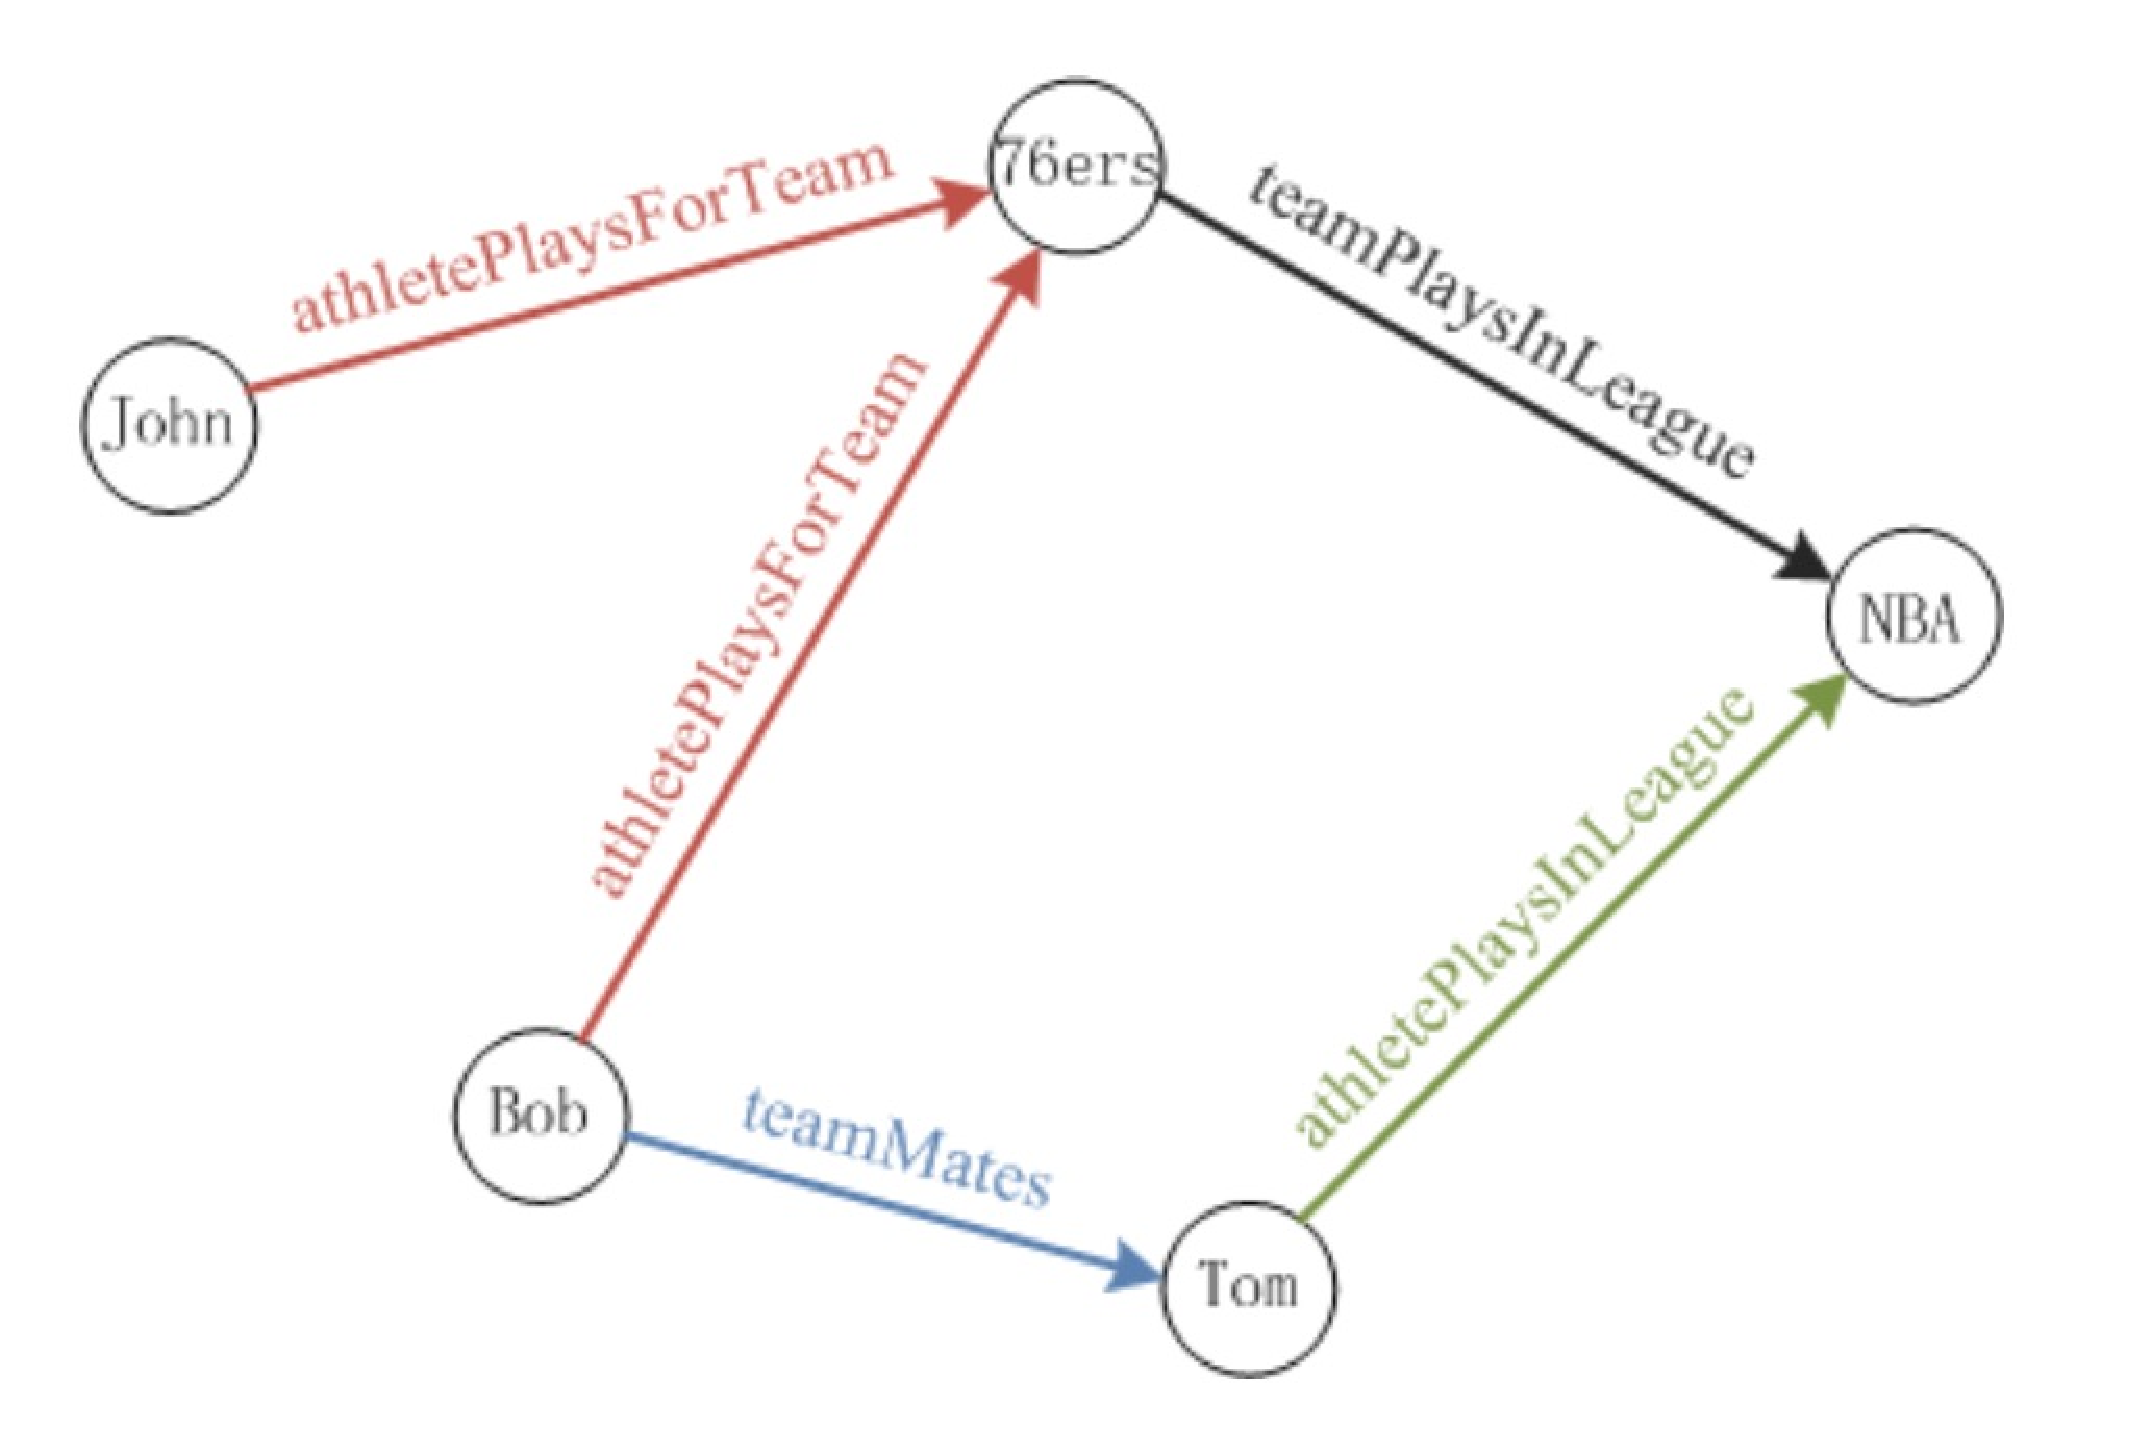
\includegraphics[width=.85\textwidth]{2.eps}
			\end{figure}
		\end{column}
		\begin{column}{0.45\textwidth}
			\begin{itemize}
			\begin{tiny}
				\item (John, athletePlaysForTeam, 76ers)
				\item (Bob, athletePlaysForTeam, 76ers)
				\item (Tom, athleteMates, Tom)
				\item (Tom, athletePlaysInLeague, NBA)
				\item (76ers, teamPlaysInLeague, NBA)
			\end{tiny}
			\end{itemize}
		\end{column}
	\end{columns}
	\item However the knowledge graph is incomplete: it only covers small part of facts.
	\end{itemize}
\end{frame}

\subsection{Knowledge Inference}
\begin{frame}
\frametitle{Knowledge Inference}
\begin{itemize}
	\item Knowledge inference: link prediction in knowledge graph.

	\begin{columns}[onlytextwidth]
		\begin{column}{0.45\textwidth}
			\begin{figure}
				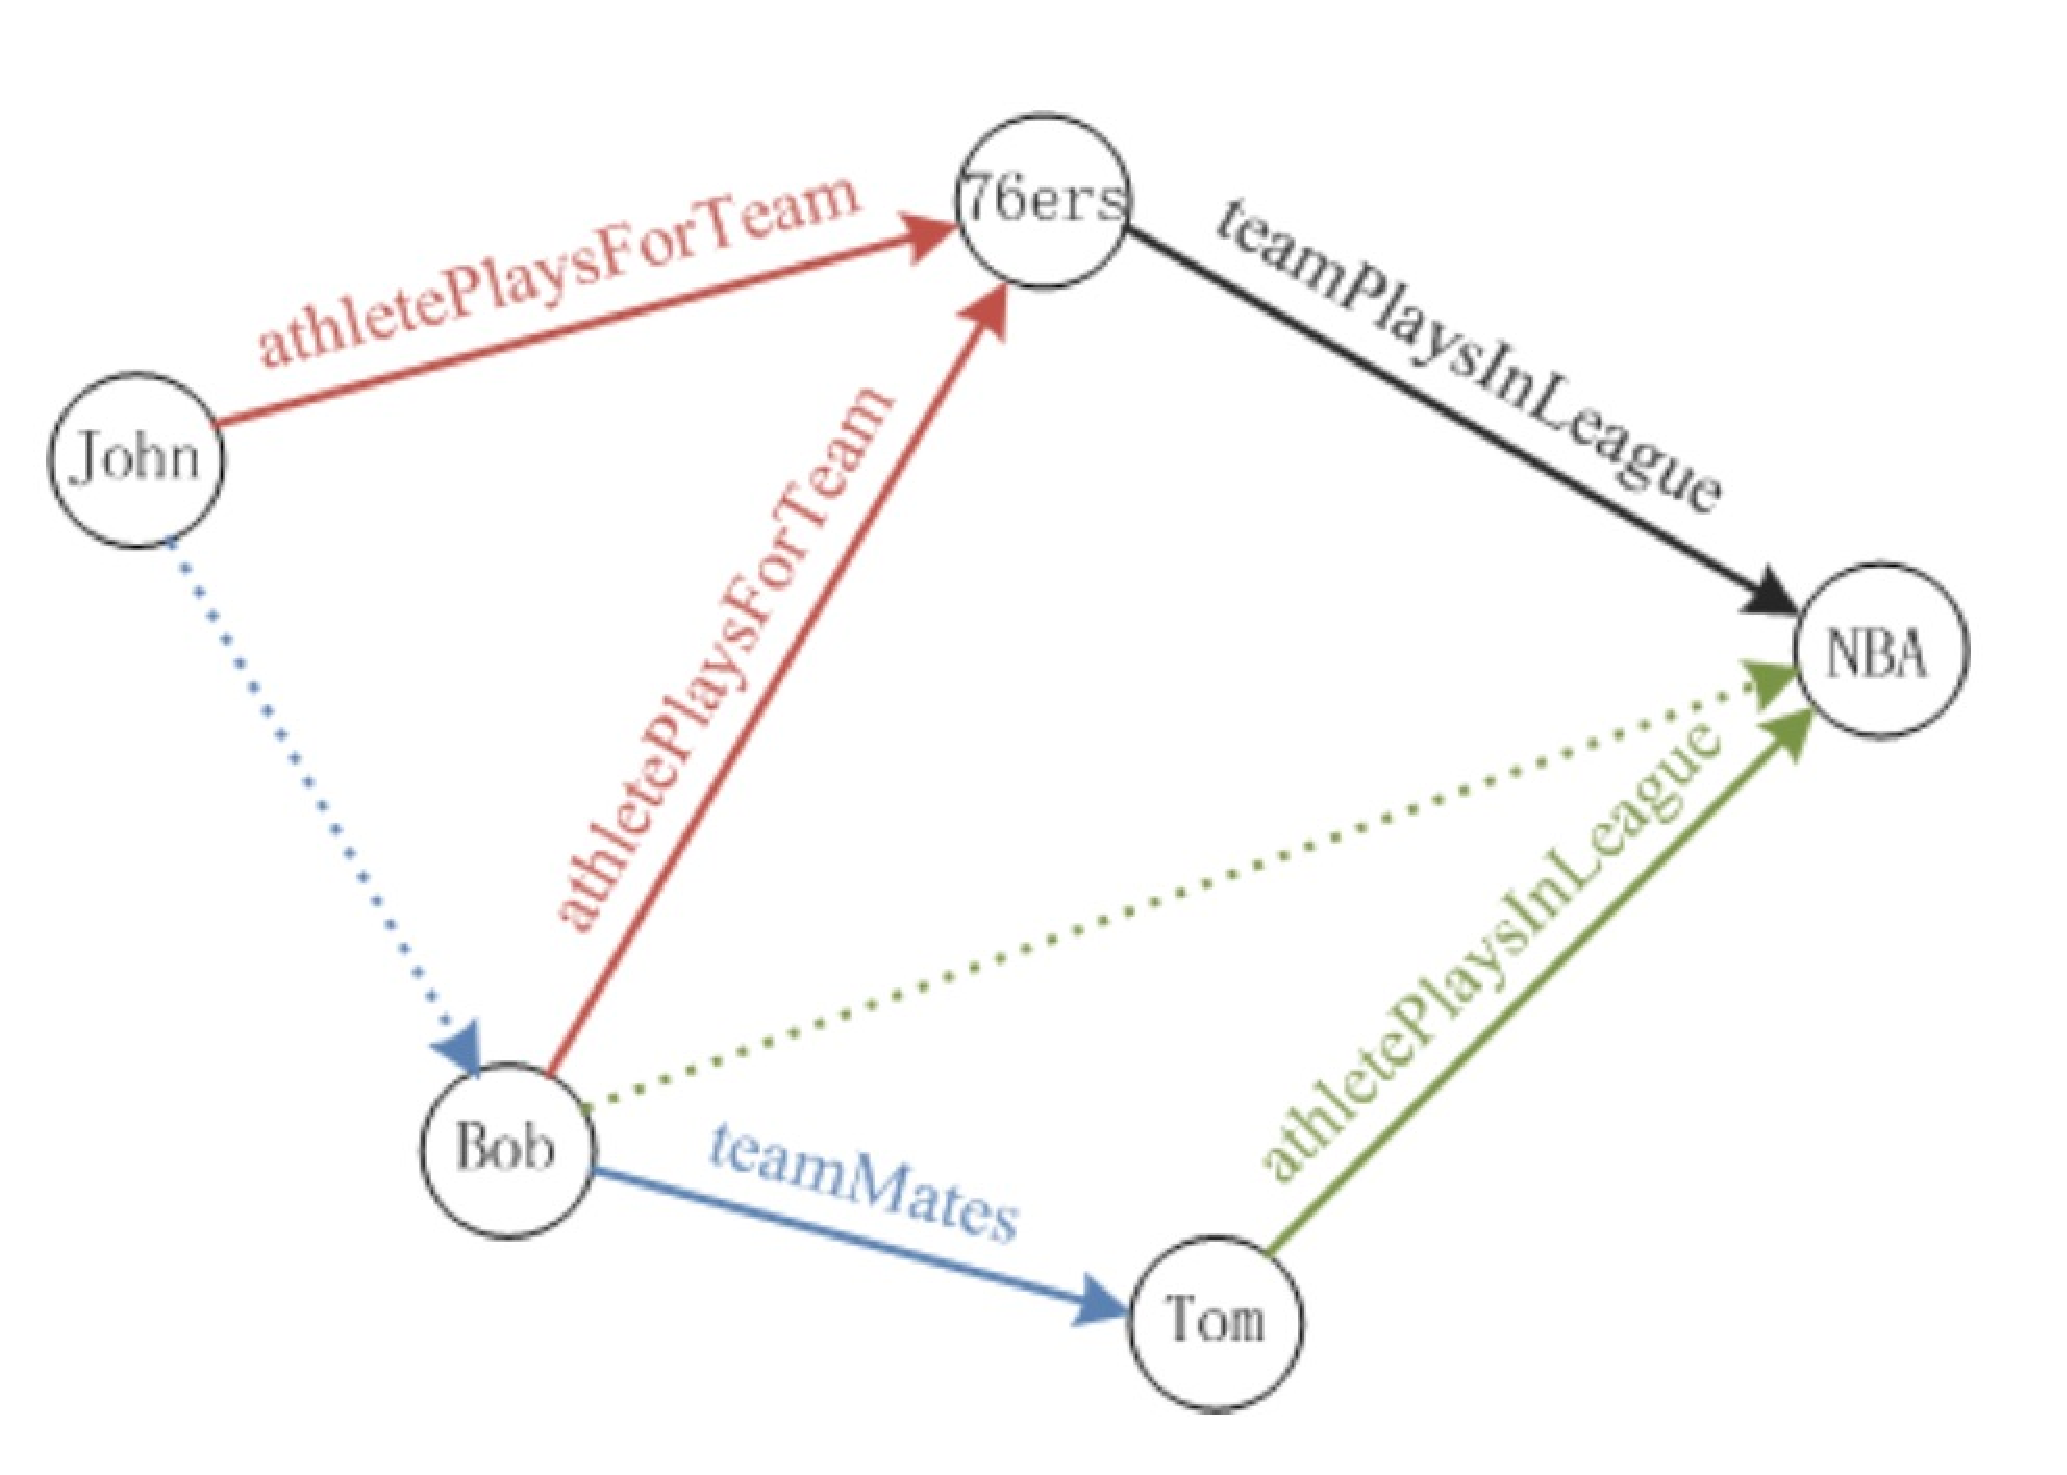
\includegraphics[width=.85\textwidth]{4.eps}
			\end{figure}
		\end{column}
		\begin{column}{0.45\textwidth}
			\begin{itemize}
			\begin{tiny}
				\item (John, teamMates, Bob)
				\item (Bob, athletePlaysInLeague, NBA)
				\item ... ...
			\end{tiny}
			\end{itemize}
		\end{column}
	\end{columns}
	\item Inference in Knowledge Graph can increase the coverage.
\end{itemize}
\end{frame}

\subsection{Methods}
\begin{frame}
\frametitle{Methods}
\begin{itemize}
	\item Inference based on representation learning.
		\begin{enumerate}
			\item Collective Matrix Factoriation \citep{nickel2011three}
			\item Neural Tensor Networks \citep{socher2013reasoning}
			\item Translating Embeddings\citep{bordes2013translating}
		\end{enumerate}
	\item Inference based on markov random field.
		\begin{enumerate}
			\item Markov Logic Networks \citep{richardson2006markov}
			\item Probabilistic Soft Logic \citep{brocheler2012probabilistic}
		\end{enumerate}
	\item Inference based on random walk.
		\begin{enumerate}
			\item Path Ranking \citep{lao2011random}
		\end{enumerate}
\end{itemize}
\end{frame}

\section{Representation Learning for Knowledge Graph}

\subsection{Framework}
\begin{frame}
	\frametitle{Framework}
	\begin{itemize}
		\item Hidden variable model: modeling data in hidden variable space.
	\end{itemize}
	\begin{block}{Leanring}
		\begin{itemize}
			\item Learning entity and relation embeddings in hidden vector spaces.
			\item Define a fitness funtion to determine the certainty of entity-relation-entity pairs.
			\item Define an objective funtion and use the facts dataset to learn the model parameters.
		\end{itemize}
	\end{block}
	\begin{alertblock}{Prediction}
		\begin{itemize}
			\item Using the model and objective function to inference.
		\end{itemize}
	\end{alertblock}
\end{frame}

\begin{frame}
	\frametitle{Framework}
	\begin{itemize}
		\item Hidden variable model: modeling data in hidden variable space.
	\end{itemize}
	\begin{block}{Leanring}
		\begin{itemize}
			\item Learning entity and relation embeddings in hidden vector spaces.
			\item Define a fitness funtion to determine the certainty of entity-relation-entity pairs.
			\item Define an objective funtion and use the facts dataset to learn the model parameters.
		\end{itemize}
	\end{block}
	\begin{alertblock}{Objective function}
		\begin{itemize}
			\item Reconstruction error
			\item Ranking loss
		\end{itemize}
	\end{alertblock}
\end{frame}

\subsection{Methods based on Reconstruction Error}
\begin{frame}
\frametitle{RESCAL: reconstruction error}
\begin{itemize}
	\item Representation in hidden vector/matrix space and the corresponding fitness function:
		\begin{figure}
			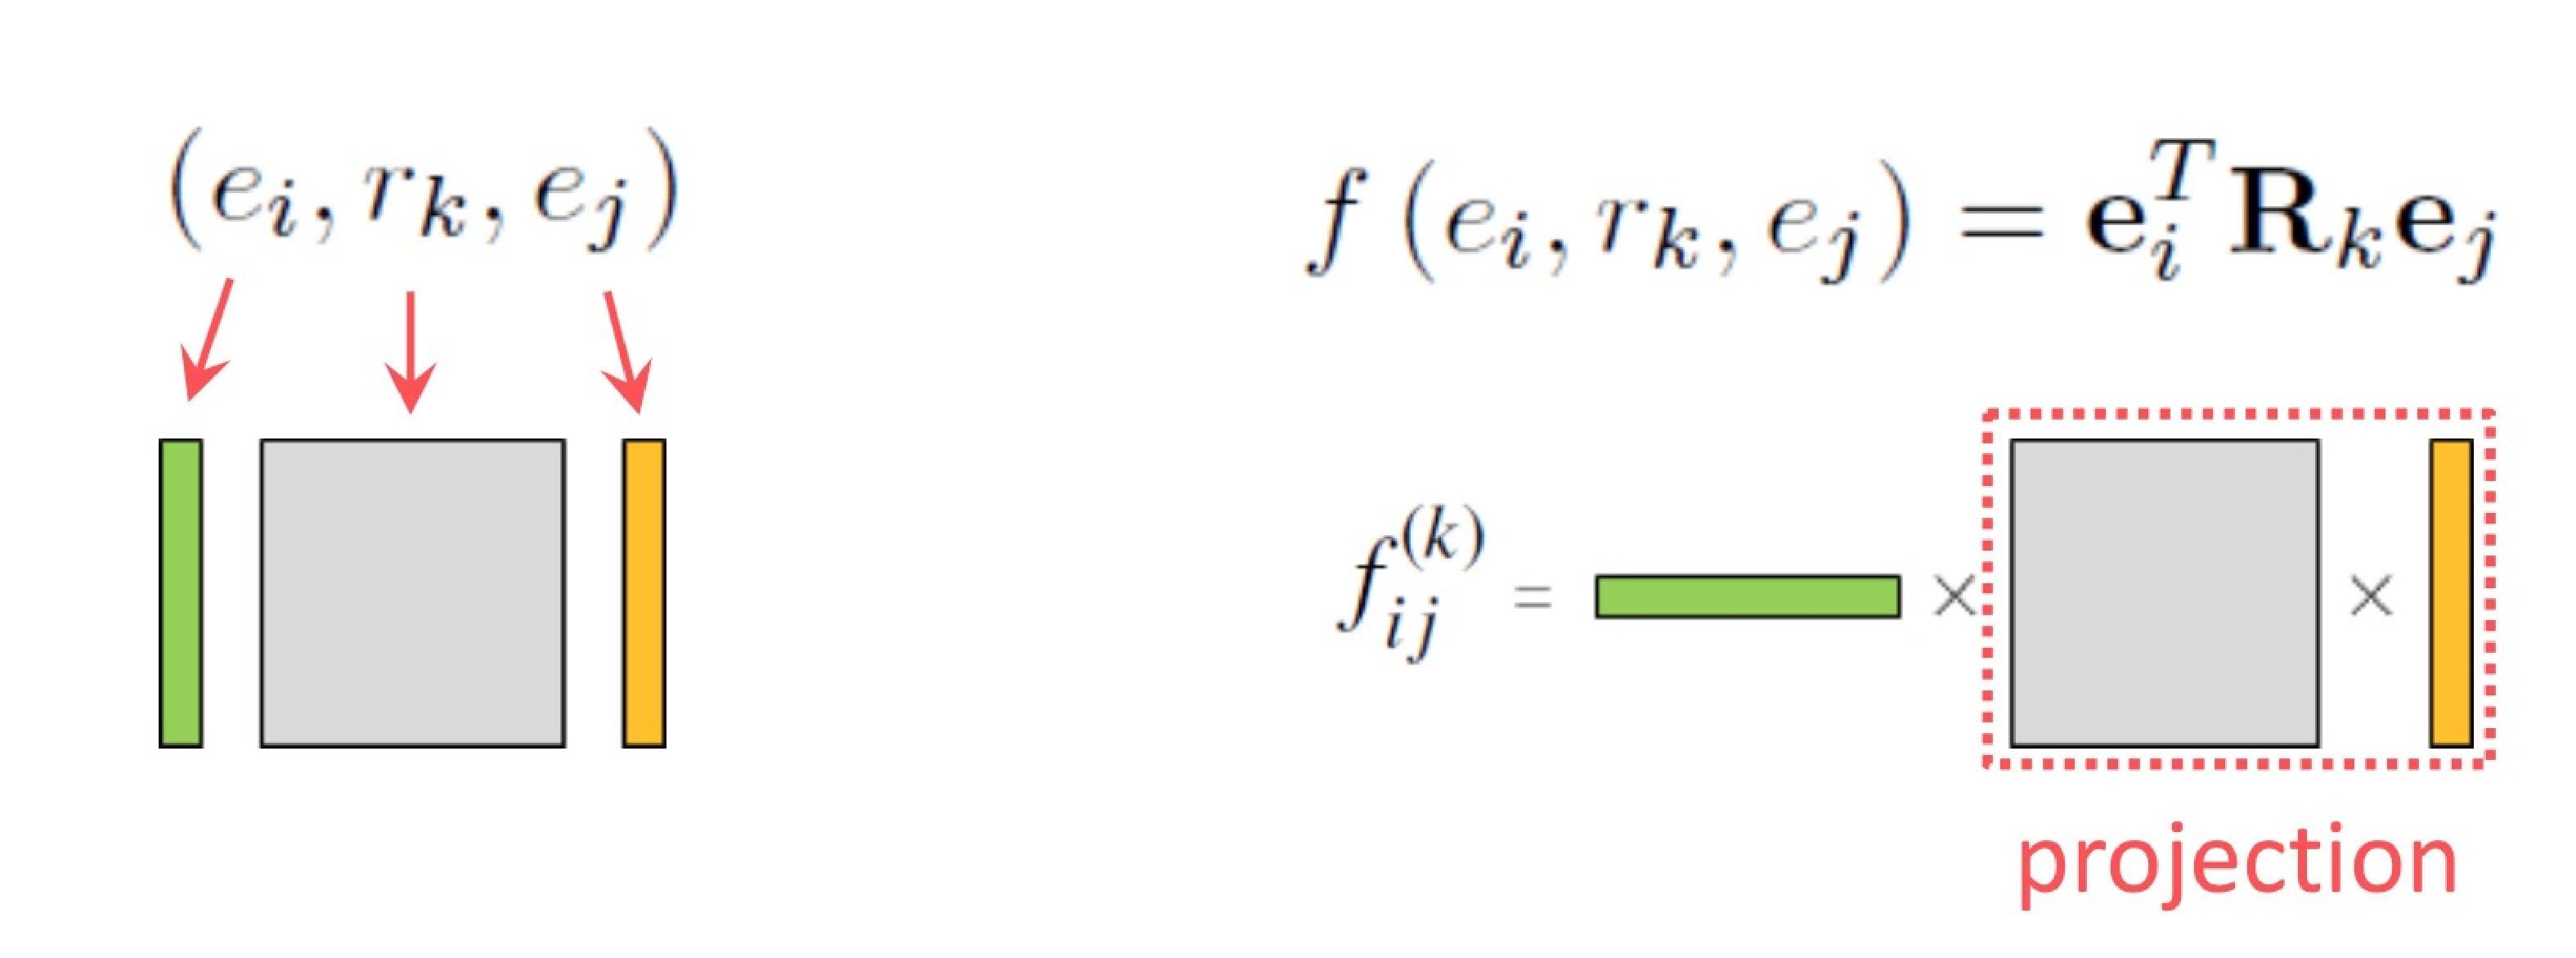
\includegraphics[height=0.20\textwidth]{5.eps}
		\end{figure}
	\item Learn based on reconstruction error:
		$$\min_{e_i,R_k}\sum_k\sum_i\sum_j{(y_{i,j}^k-f(e_i,r_k,e_j))^2+\lambda R}$$
	\begin{exampleblock}{assumption}
		It is assumed that all pairs not contained in dataset are negative.
	\end{exampleblock}
\end{itemize}
\end{frame}

\subsection{Methods based on Ranking Loss}
\begin{frame}
\frametitle{Neural Tensor Network: ranking loss}
\begin{itemize}
	\item Representation in hidden vector/matrix space and the corresponding fitness function:
		\begin{figure}
			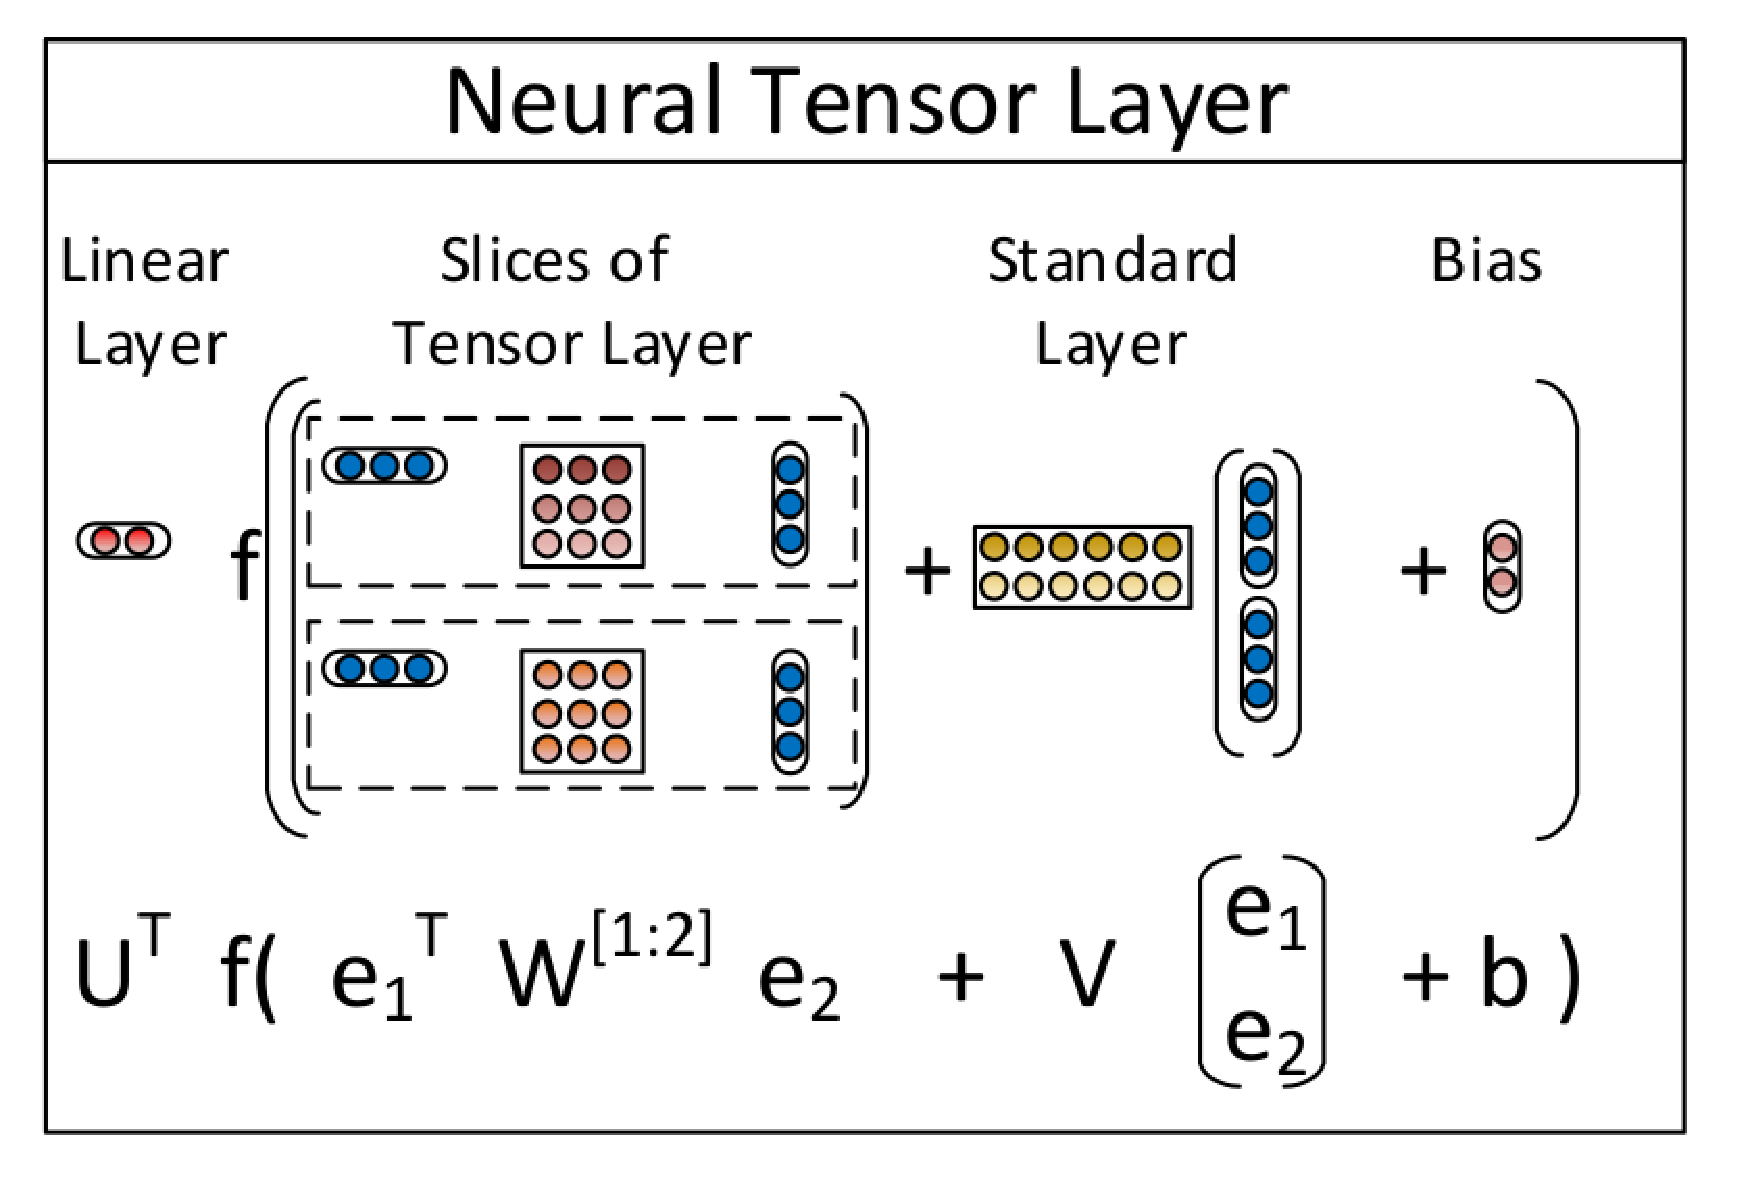
\includegraphics[width=0.60\textwidth,height=0.30\textwidth]{7.eps}
		\end{figure}
		$$f(e_i,r_k,e_j)=U_k^Tg(e_i^TW_k^{[1:K]}e_j + V_k[e_i:e_j] + b_k)$$
	\item Learn based on ranking loss:
		$$\min_{e_i,R_k}\sum_{t^+ \in O}\sum_{t^- \in D}{(\lambda + f(e_i,r_k,e_j) - f(e'_i,r_k,e'_j))}$$
	\begin{exampleblock}{assumption}
		It is assumed that all pairs not contained in dataset are negative.
	\end{exampleblock}
\end{itemize}
\end{frame}

\begin{frame}
\frametitle{TransE: ranking loss}
\begin{itemize}
	\item Representation in hidden vector space and the corresponding fitness function:
		\begin{figure}
			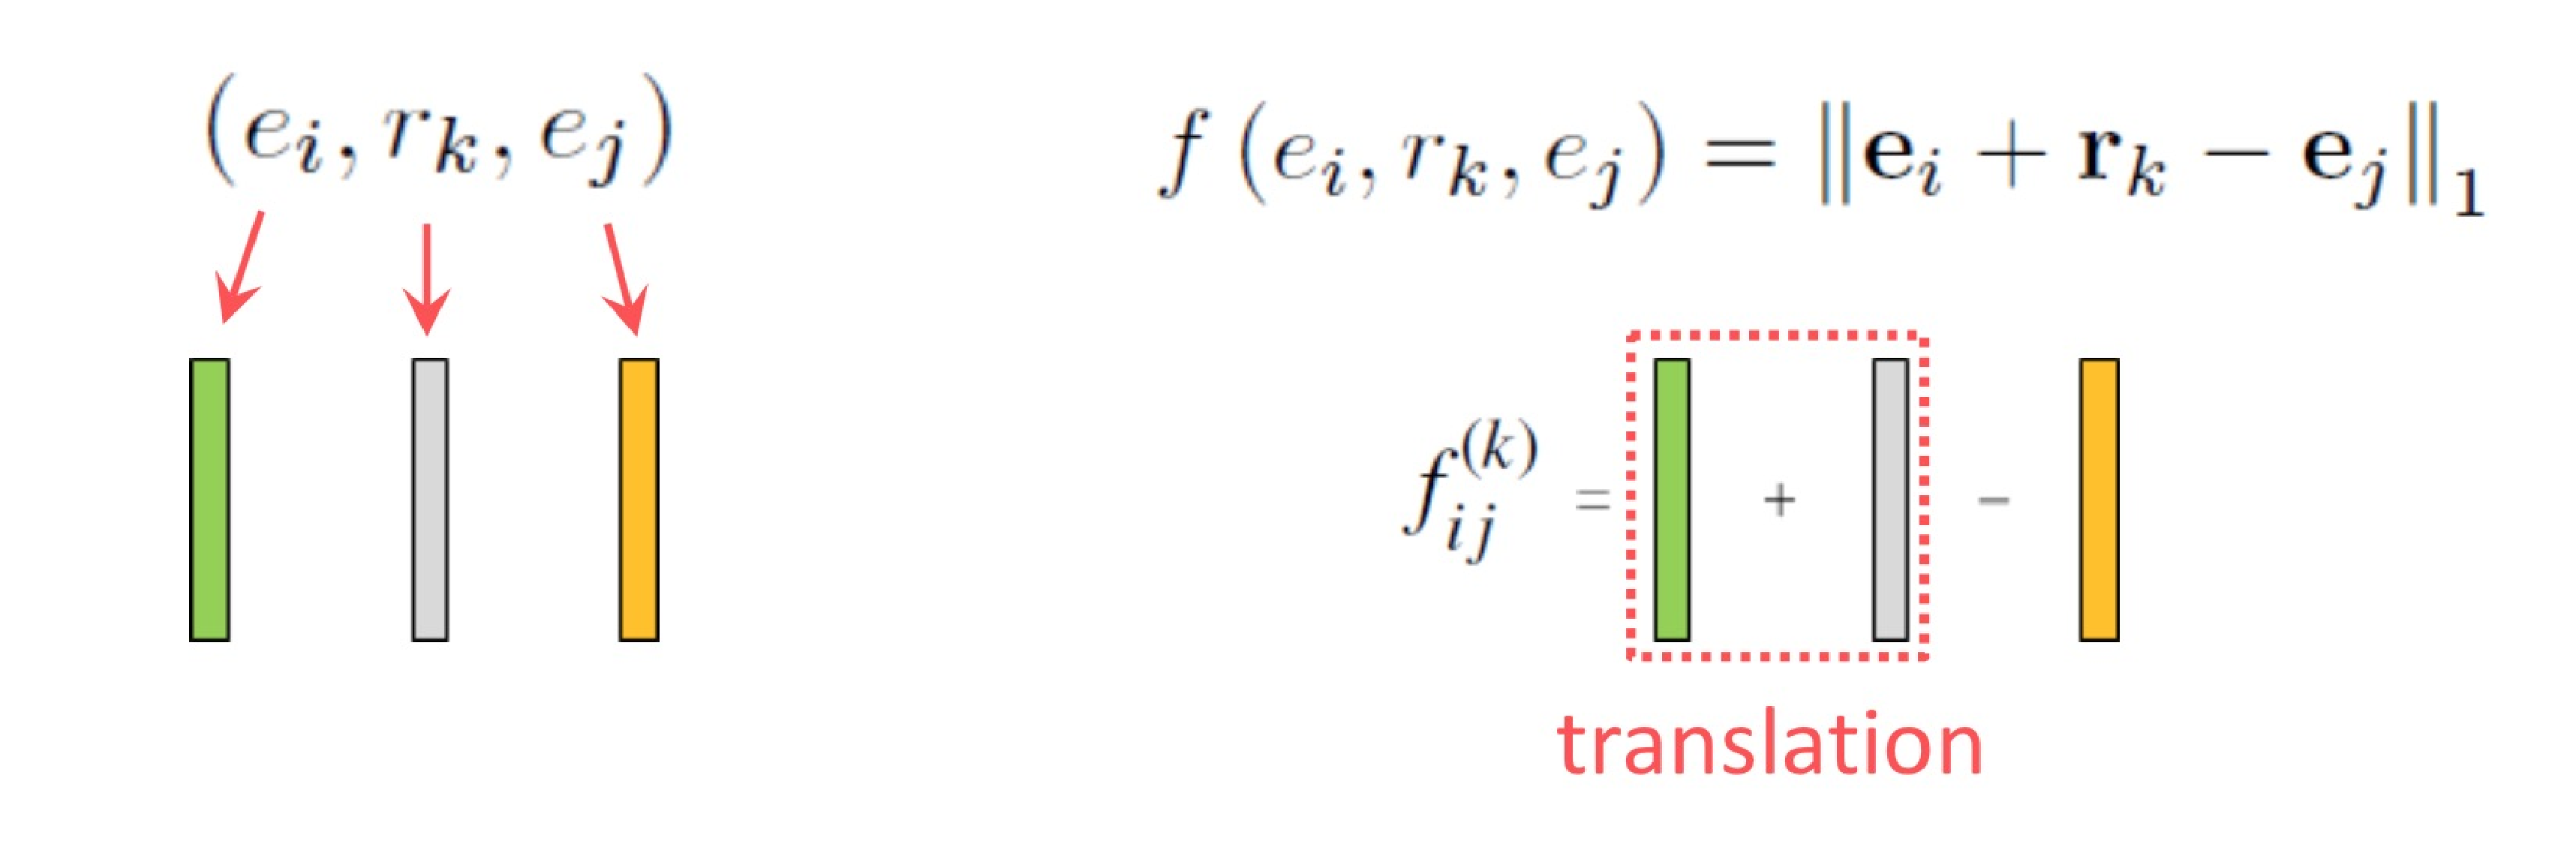
\includegraphics[height=0.20\textwidth]{6.eps}
		\end{figure}
	\item Learn based on ranking loss:
		$$\min_{e_i,R_k}\sum_{t^+ \in O}\sum_{t^- \in D}{(\lambda + f(e_i,r_k,e_j) - f(e'_i,r_k,e'_j))}$$
	\begin{exampleblock}{assumption}
		It is assumed that pairs not contained in dataset are partially negative.
	\end{exampleblock}
\end{itemize}
\end{frame}

\section{Our Idea: Combine Knowledge with Mention}

\begin{frame}
\frametitle{Motivation}
    \begin{itemize}
        \item All pages above describes the recent representative  learning in knowledge graph field. In this section we briefly introduce our work.
        \item In the information extraction field, one may have the information both from knowledge graph and text mention. They together can give more confidence in the relation inference.
        \item Our idea is to build a model which can utilize both knowledege graph and mentions jointly to determine the relation type.
    \end{itemize}
\end{frame}

\begin{frame}
    \frametitle{Motivation}
    \begin{itemize}
        \item Formally, if given the dataset not only with entity and relation tuple $(e_1, r, e_2)$, but also the text mention $m$ about the relation, can we adopt the information to enhance the inference precision?
        \item This is the problem that this work is to figure out.
    \end{itemize}
\end{frame}

\section{Data}
\begin{frame}
\frametitle{Data Preparation}
    \begin{itemize}
        \item Luckily the NELL dataset contains the evidence when NELL system extract this tuple from the website. We can use the evidence as the relation mention in our work.
        \item We process the NELL dataset and extract available portion with mention as our experiment dataset. The sample in dataset has a format with $(e_1, r, e_2, m)$.
        \item The prepared  dataset has 34245 entities and 233 relations, each row has word sequance as relation mention.
    \end{itemize}
\end{frame}

\section{Model}
\begin{frame}
    \frametitle{Mention Loss}
    \begin{itemize}
        \item We use TransE model as our basic model. In addition to TransE loss, we add mention loss function to be minimized. Similarly, we use the hinge loss about the mentions:
            $$L_m=[D(g(m), r) + 1 - D(g(m), r')]_+$$
        \item where $g$ is the function to transfer mention into a vector and $D(\dot)$ measure the distance between $g(m)$ and $r$. 
        \item We want the mention to produce the similar vector as $r$. 
    \end{itemize}
\end{frame}

\begin{frame}
    \frametitle{Mention Model}
    \begin{itemize}
        \item In our implementation the advanced relation extraction CNN model\citep{zeng2014relation} is used.
            \begin{figure}
				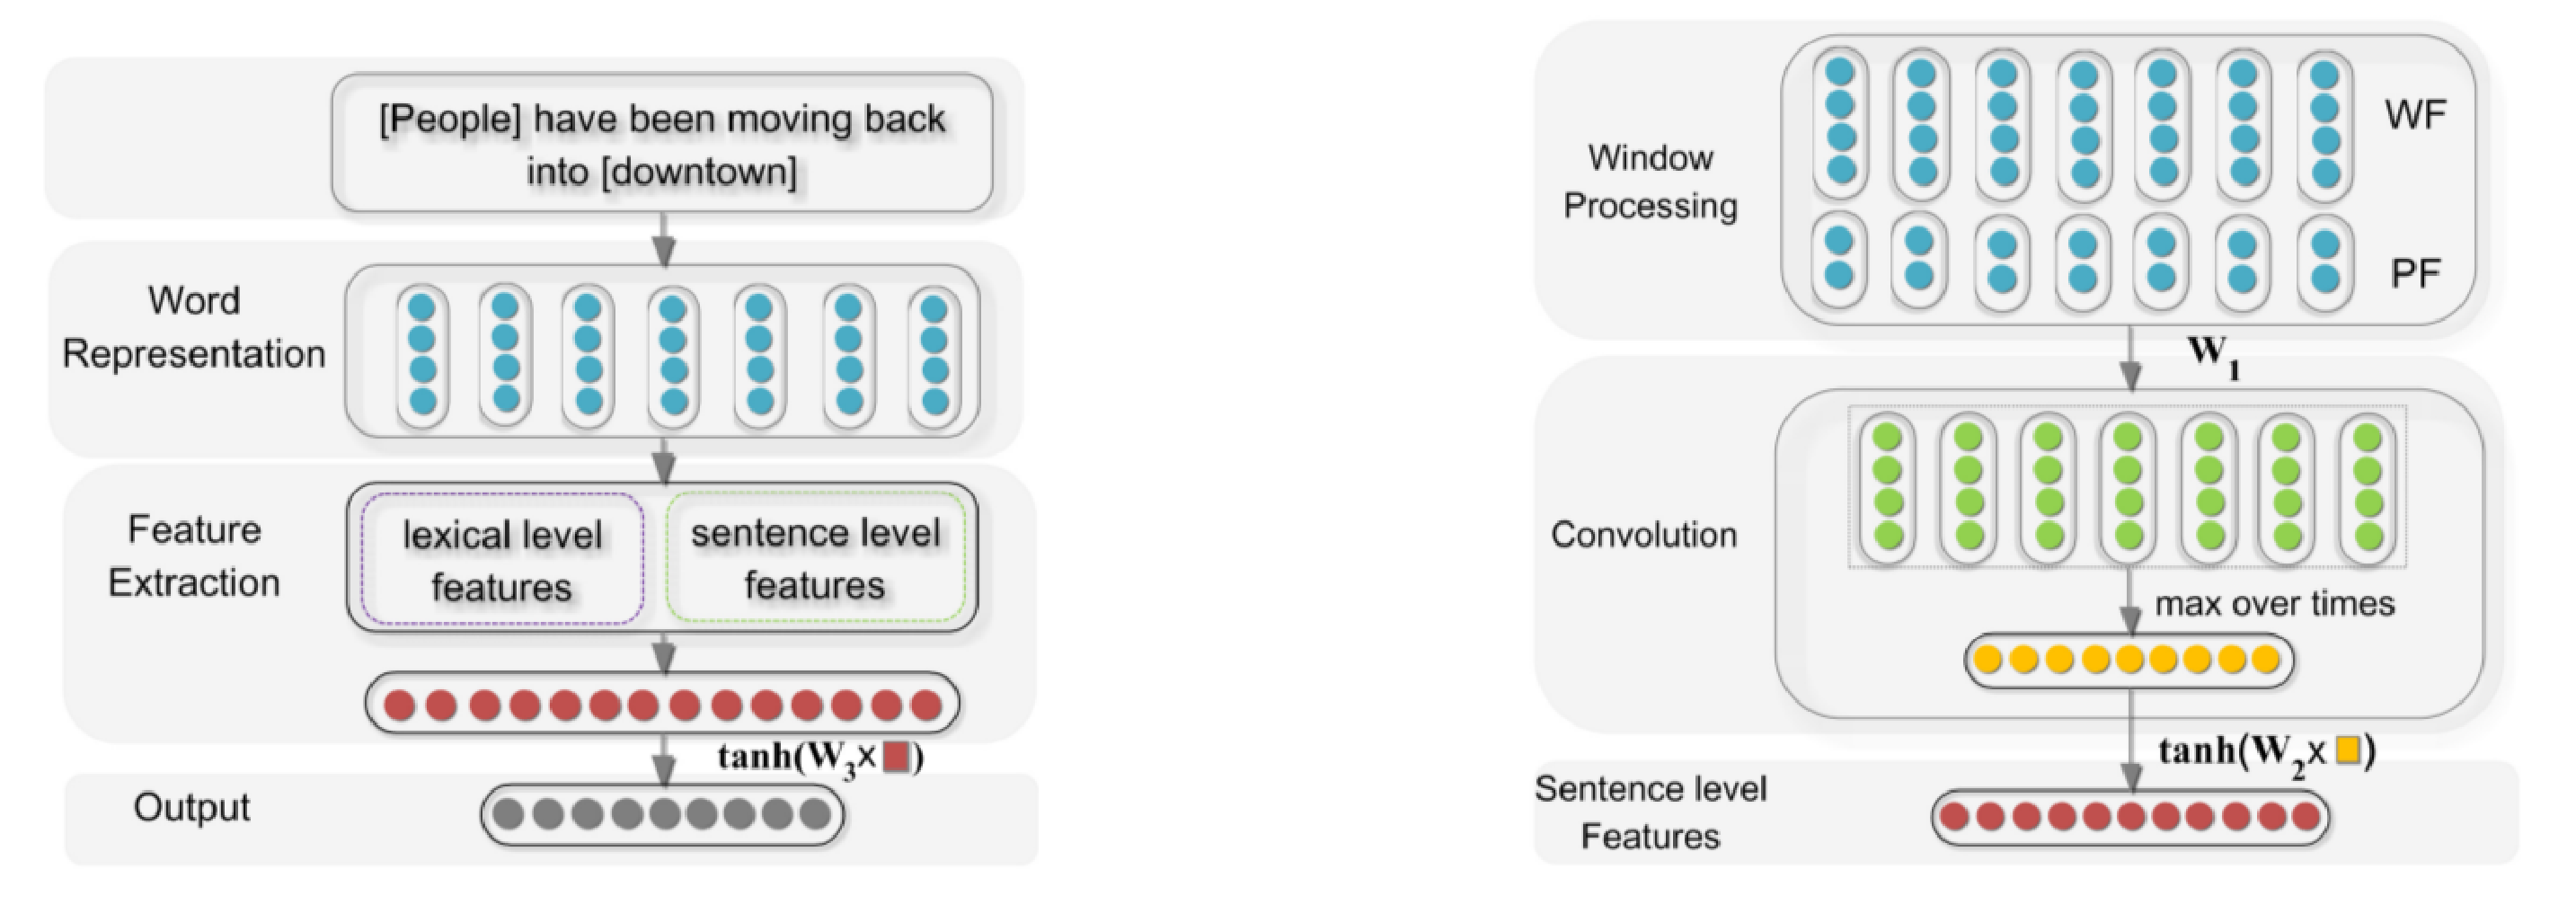
\includegraphics[width=.85\textwidth]{10.eps}
            \end{figure}
        \item The framework keeps the same in his paper but we omit the lexical feature as entity mention is not included in NELL dataset and we modify the last layer to be simple fully connected layer rather than a softmax layer as it is not a classification task.
    \end{itemize}
\end{frame}

\section{Result}
\begin{frame}
\frametitle{Experiment and Result}
    \begin{itemize}
        \item We evaluate the performance of TransE with or without mention information to see how much it can improve.
        \item Here we choose the mean rank measurement in testing. Mean rank measure the ranks of true relation among all relation candidates and average them.
    \begin{table}[htp]
        \caption{Results of experiments}
        \begin{tabular}{c c c c}
            \hline \hline
            Case & Train $$& Valid & Test \\
            \hline
            TransE & 12.4 & 11.4 & 13.4 \\
            TransE-mention & 3.0 & 2.9 & 3.3 \\
            \hline \hline
        \end{tabular}
    \end{table}
\end{itemize}
\end{frame}

\begin{frame}[allowframebreaks]
\frametitle{References}
\bibliography{ref}
\end{frame}

\begin{frame}
	\frametitle{Thanks}
	Question \& Answer?
\end{frame}

\end{document}
